\documentclass{6042}
\usepackage{graphicx}
\graphicspath{ {./images/} }
\usepackage{tikz}
\usetikzlibrary{shapes.geometric,fit}
\graphicspath{ {./images/} }
\usepackage[linguistics]{forest}
\usepackage{braket}
\usepackage{cancel}
\usepackage{hyperref}

\author{Julius Heitkoetter}

\problemset{9}

\begin{document}

Code, data, and additional figures for this assignment can be found here: \url{https://github.com/julius-heitkoetter/particle\_physics\_statistics}

\problem{1}{None}

\textbf{NOTE:} Unless otherwise specified, the data used in this part is the \textit{small} dataset. Instead of showing my work in the writeup, I carefully documented the code in "stats\_assignment\_part1.py"

\problempart{a}

The local p-value of the peak that I see using the liklihood profile ratio as the test statistic and Wilkes theorem is $0.0485.$

\problempart{b}

The trial factor I expect using the equations we have seen is class is: 31.56.

\problempart{c}

\textbf{i} Below is the distribution of the profile likelihood under the null hypothesis as well as a blue part denoting the value of the profile liklihood found in data. I've also overlayed a red dotted line displaying a $\chi^2$ distribution with 2 degrees of freedom to demonstrate that the distribution looks like I would expect under Wilkes. 

\begin{center}
    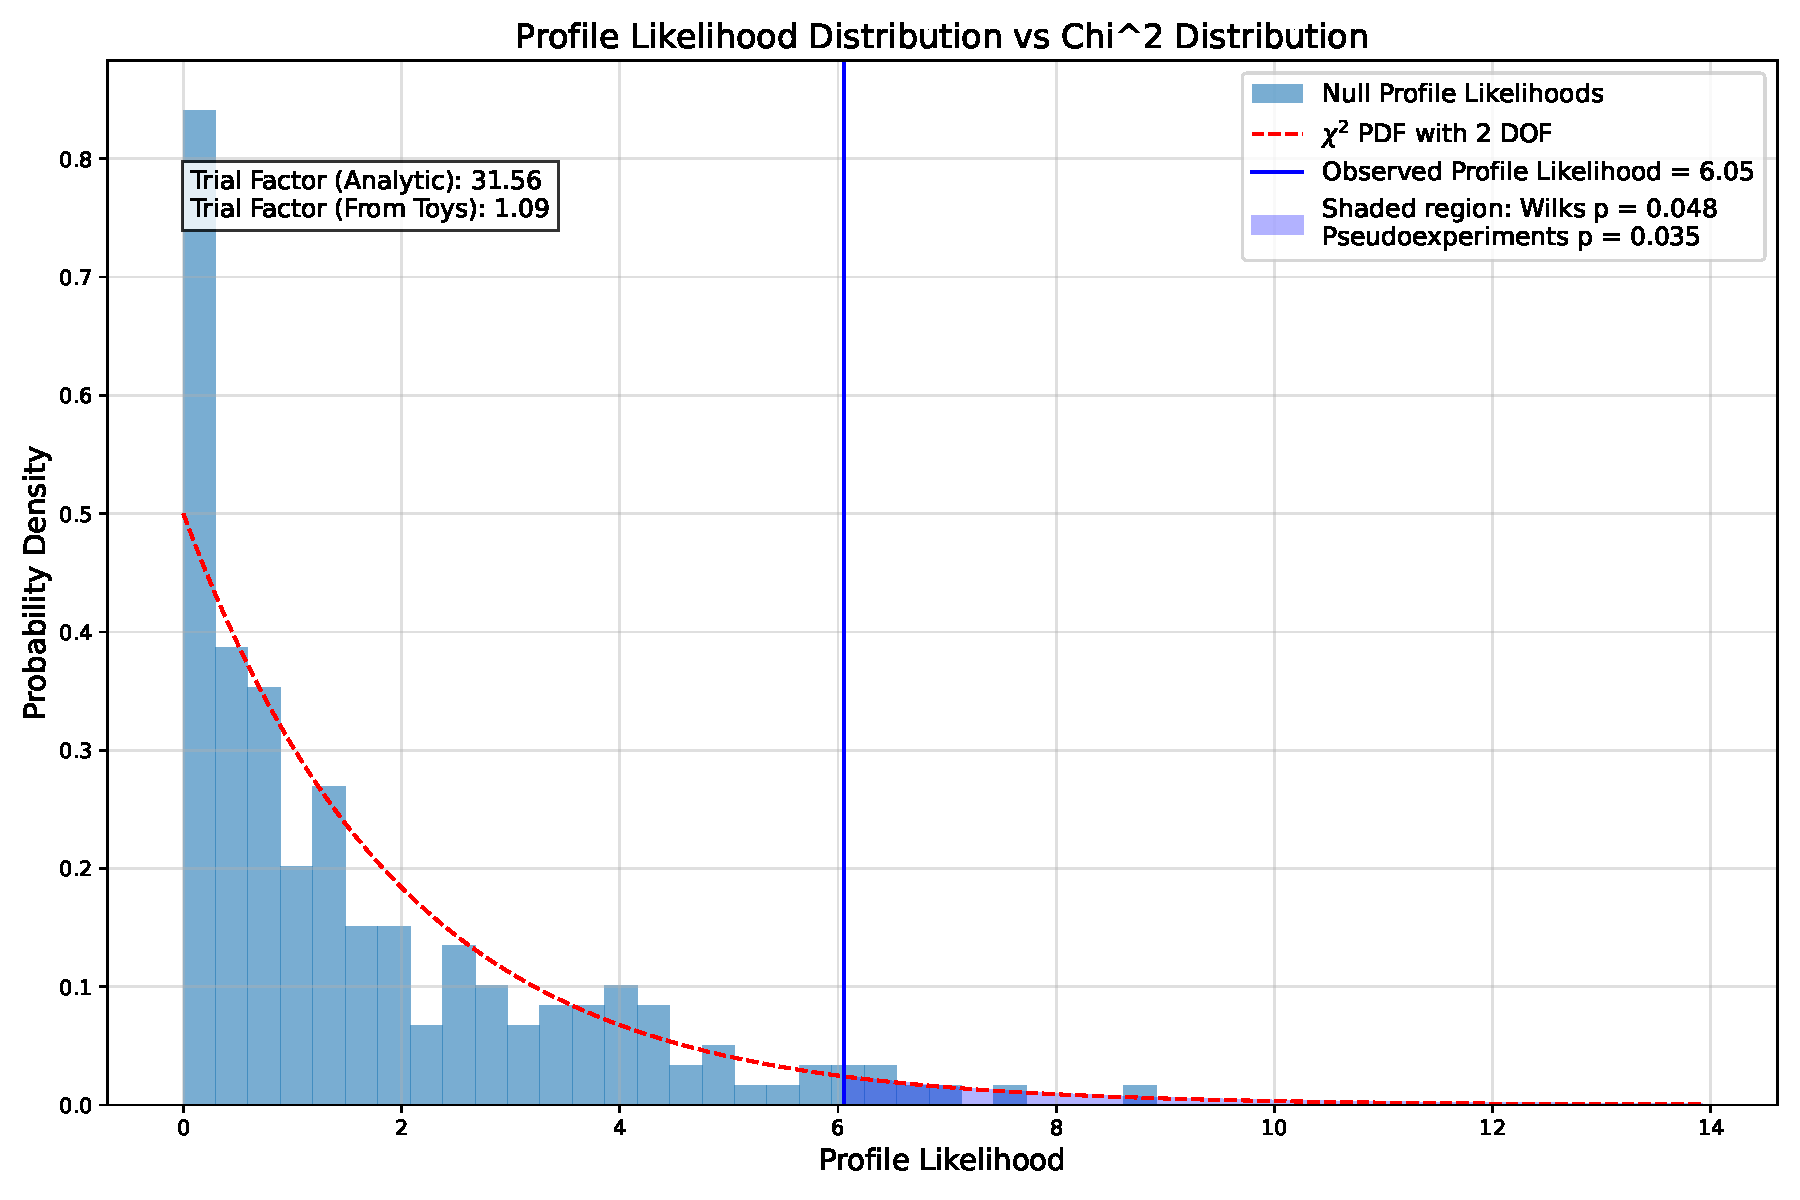
\includegraphics[scale=0.5]{images/part1_small_mMin105_mMax155/profile_liklihoods.pdf}
\end{center}

\textbf{ii} As can be read from the figure above, the p-value I got from my pseudoexperiment is $0.035$. Additionally, assuming the experiment is in the asymptotic limit, the trial factor according to the pseudo-experiments is 1.09. This can also be read off of the plot above.

\problempart{d}

The new mass range experiment should have half the trial factor of the old mass range experiment. 

When I ran the code, I got a ratio of p-values of roughly 5/8, which is farily close to the 1/2 I would have predicted. 




\problem{2}{None}

\textbf{NOTE:} Unless otherwise specified, the data used in this part is the \textit{small} dataset. Additionally, because the peak is smaller, I found it appropriate to adjust the efficiencies to be given by something less than $N_s = 45 \times \mu$. After doing an initial couple fits, I decided to instead test for $N_s = 22 \times \mu$. However, you can find in the git repo the figures associate with $N_s = 45 \times \mu$ under the "figures" directory.

\problempart{a}

Below is the plot of the profile likelihood test statistic under the signal and background hypothesis under several different mass bins. 200 toys were used. 

\begin{center}
    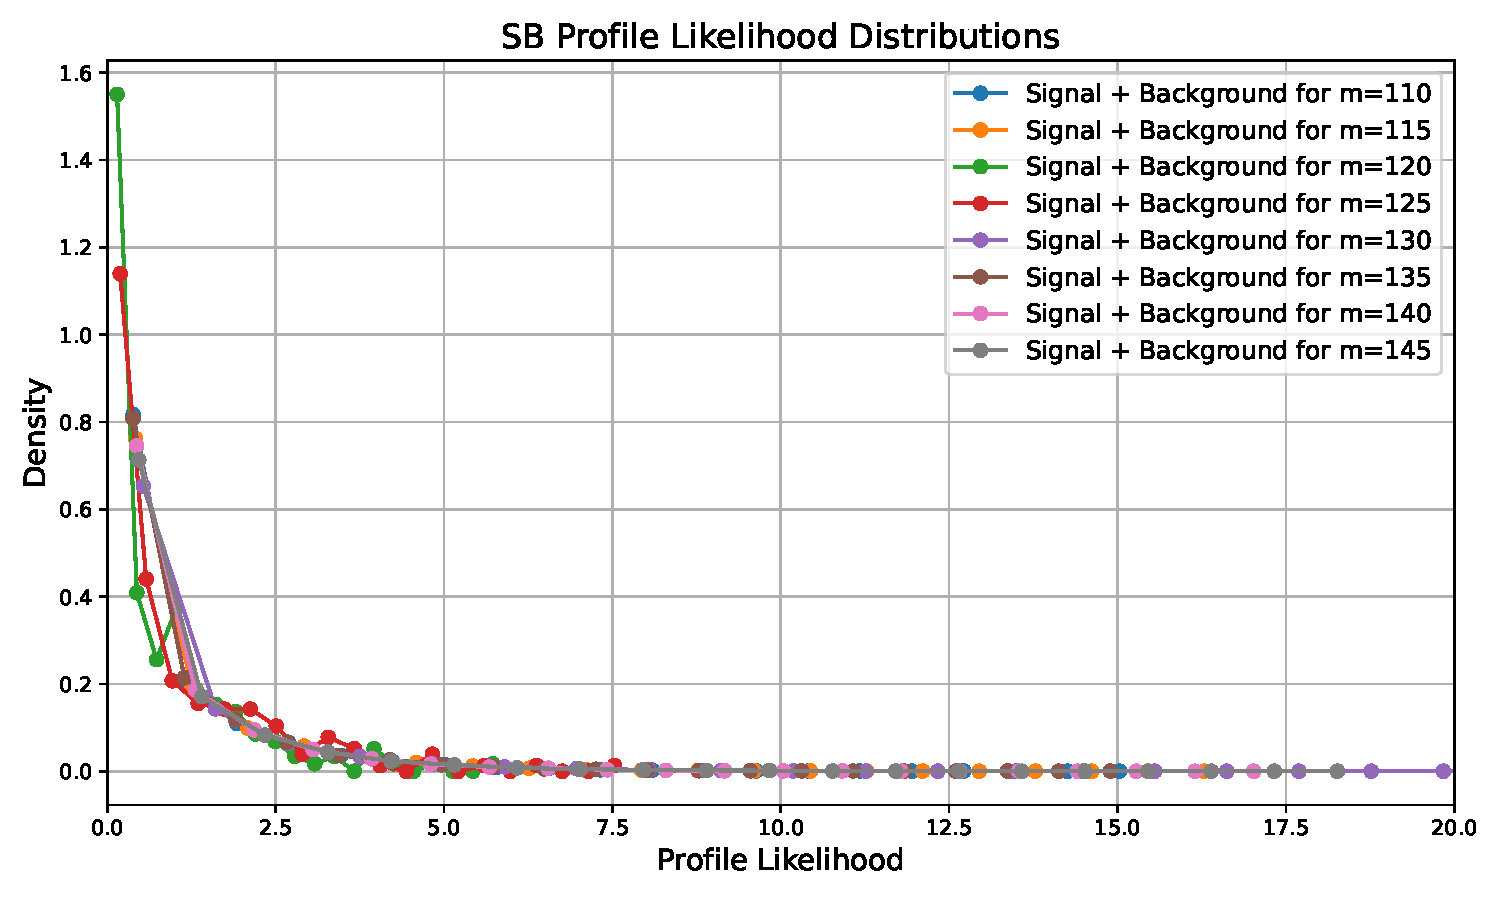
\includegraphics[scale=0.5]{images/cls_small_nsig22/cls_sb_profile_likelihoods_mass_binned.pdf}
\end{center}

\problempart{b}

Below is the plot of the profile likelihood test statistic under the background only hypothesis under several different mass bins. 

\begin{center}
    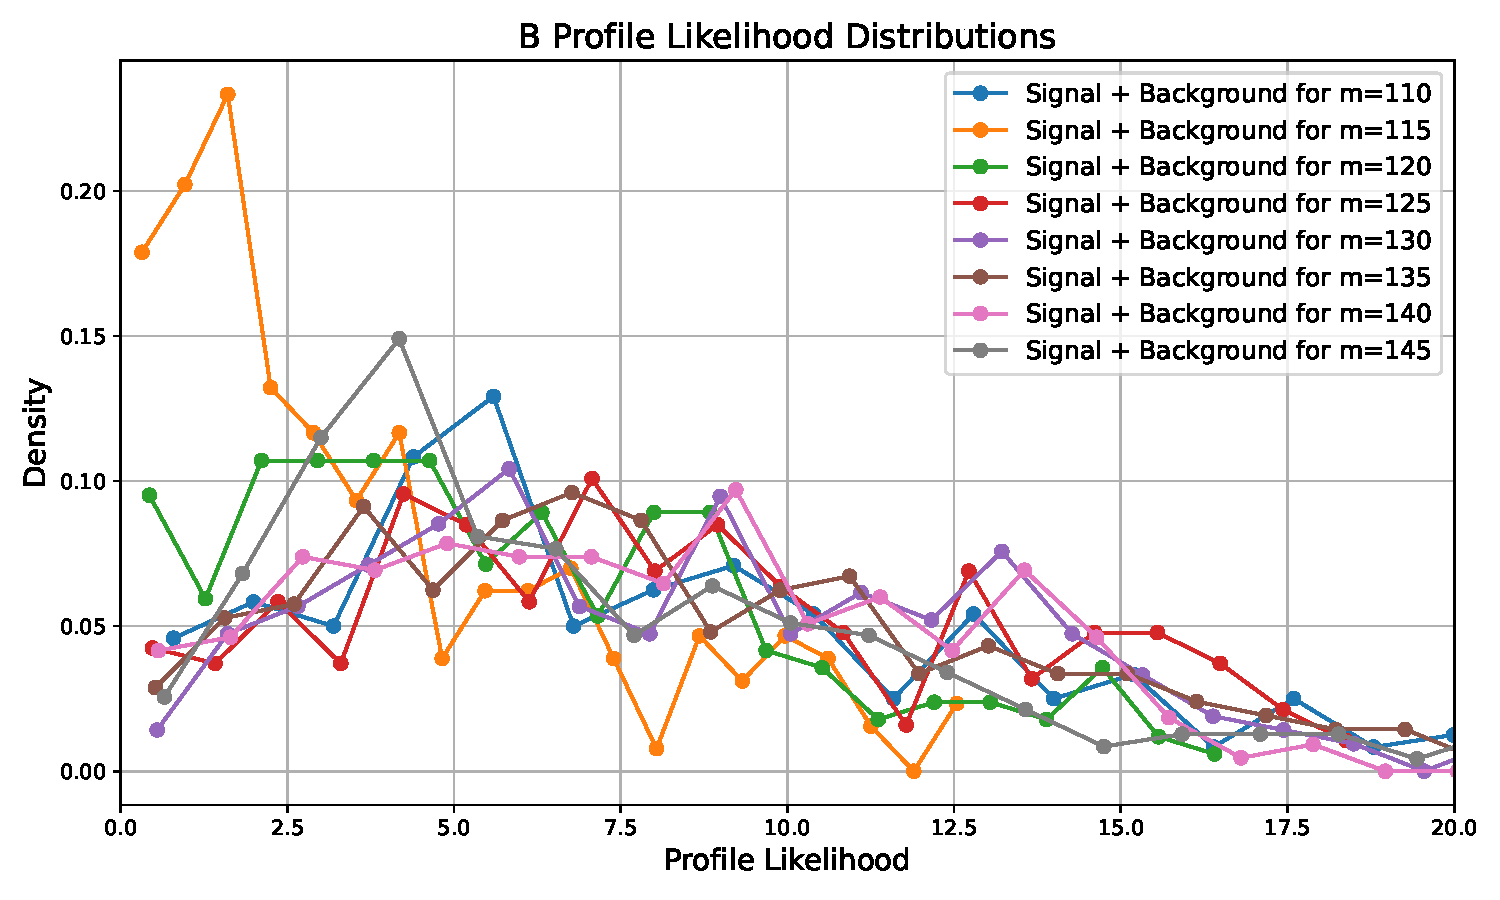
\includegraphics[scale=0.5]{images/cls_small_nsig22/cls_b_profile_likelihoods_mass_binned.pdf}
\end{center}

As you can see, the test statistic generated under the background only hypothesis is not dependent on the mass, $m_{SM}$, because the fit parameters are independent of the mass parameter. It is, however, quite noisy, even though 200 toys were used. 

\problempart{c}

Below you can see the profile likelihood distribution for the background only and signal+background hypothesis, for the $m_{SM} = 120$ GeV bin. 

The green line represents a confidence level of $0.05$ with respect to the signal+background hypothesis. We then use the background only hypothesis to calculate the power as $0.74$.

\begin{center}
    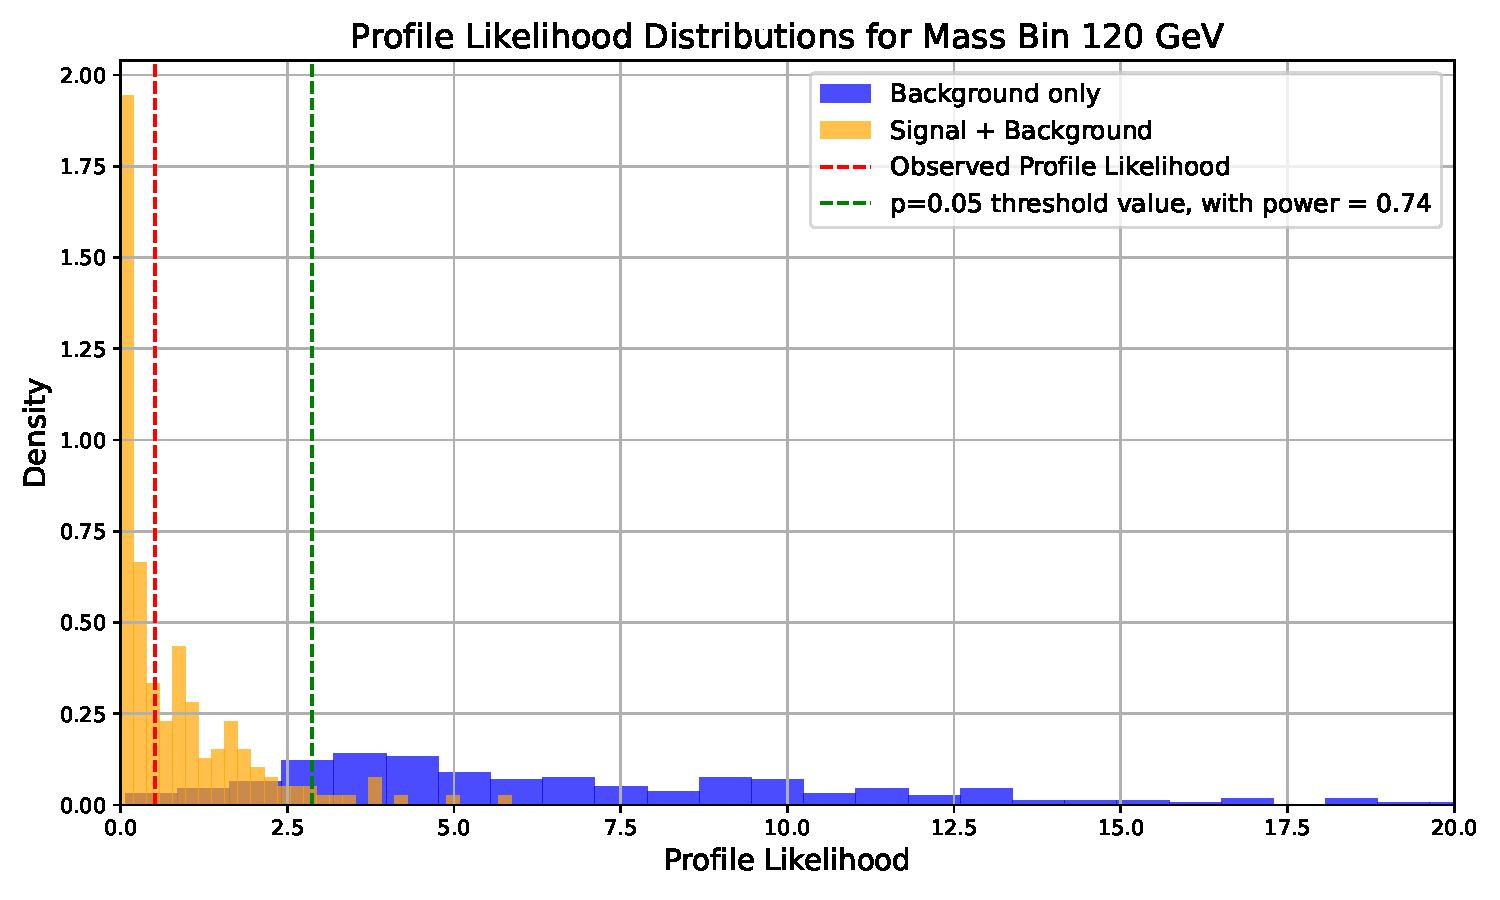
\includegraphics[scale=0.5]{images/cls_small_nsig22/cls_profile_liklihood_distribution_m=120.pdf}
\end{center}

\problempart{d}

Below is the CLs plot generated using 200 toys

\begin{center}
    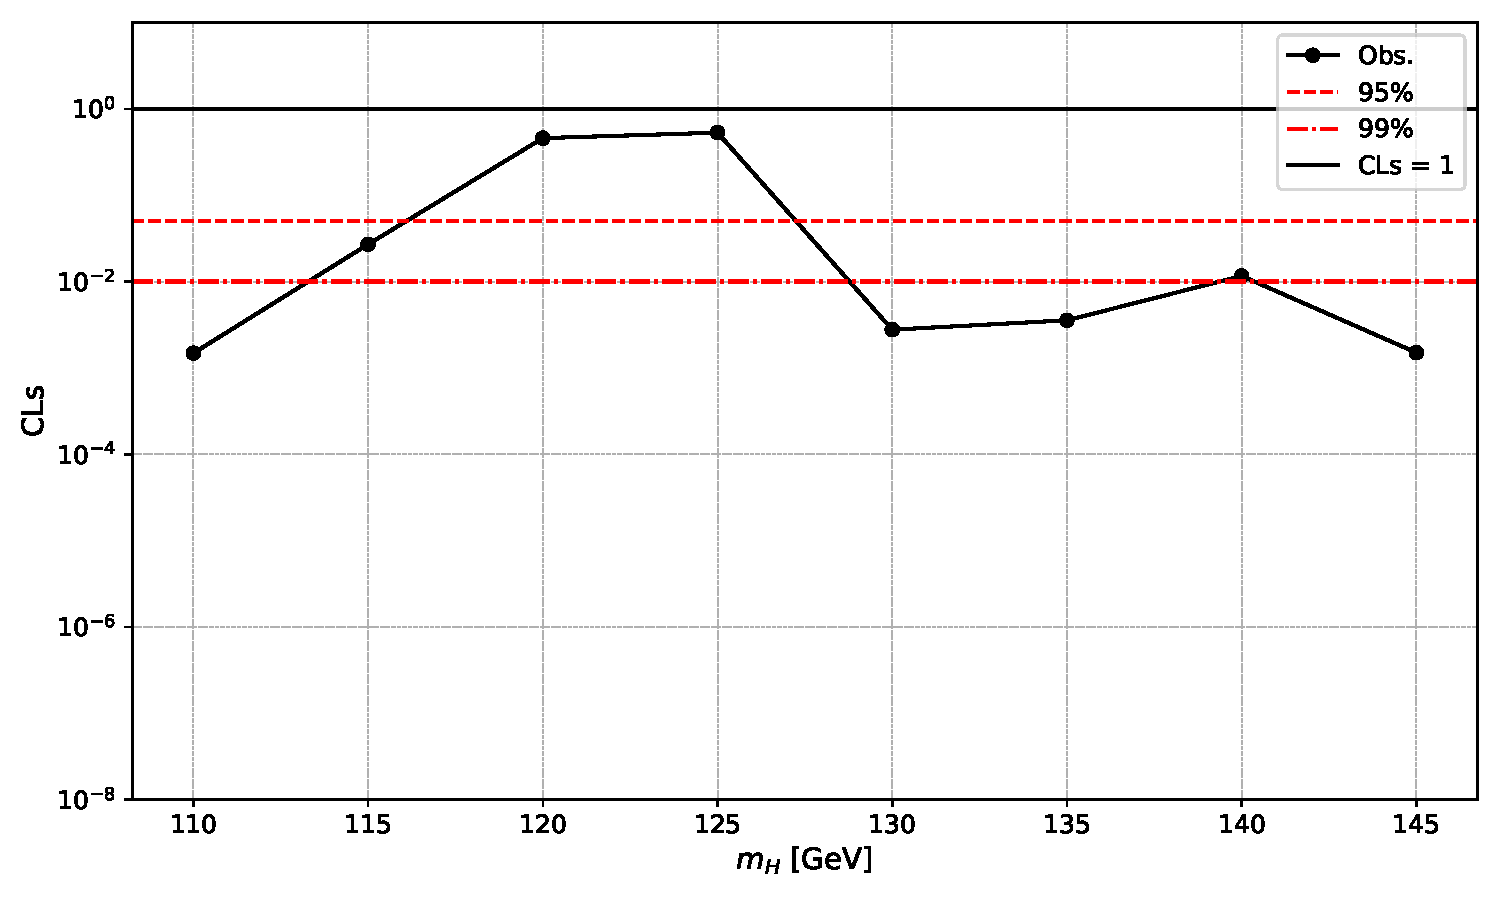
\includegraphics[scale=0.5]{images/cls_small_nsig22/cls_plot.pdf}
\end{center}

\problempart{e} 

The regions we can exclude the signal+background hypothesis safely with $95\%$ CL are: 110-115 GeV and 130-145 GeV. We cannot exclude the signal+background hypothesis safely with $95\%$ CL in the range of 115-130 GeV. This is generall the plot we'd expect since the higgs mass is around 125 GeV. 

One way to improve this plot would be with more mass bins. One way to do this efficiently, is to notice that the signal+background hypothesis follows Wilk's Theorem, and so simply can be approximated with a $\chi^2$ distribution, so we don't need to make toys for them. Furthermore, the background only hypothesis shouldn't (and isn't by inspection) dependent on the mass bin iteself, so we just need to make one set of toys. Using this, we only need to fit to the observed data per mass bin, which means it becomes much cheaper to interpolate more mass bins. 

Doing this (and using 400 toys for the background instead) gives us:

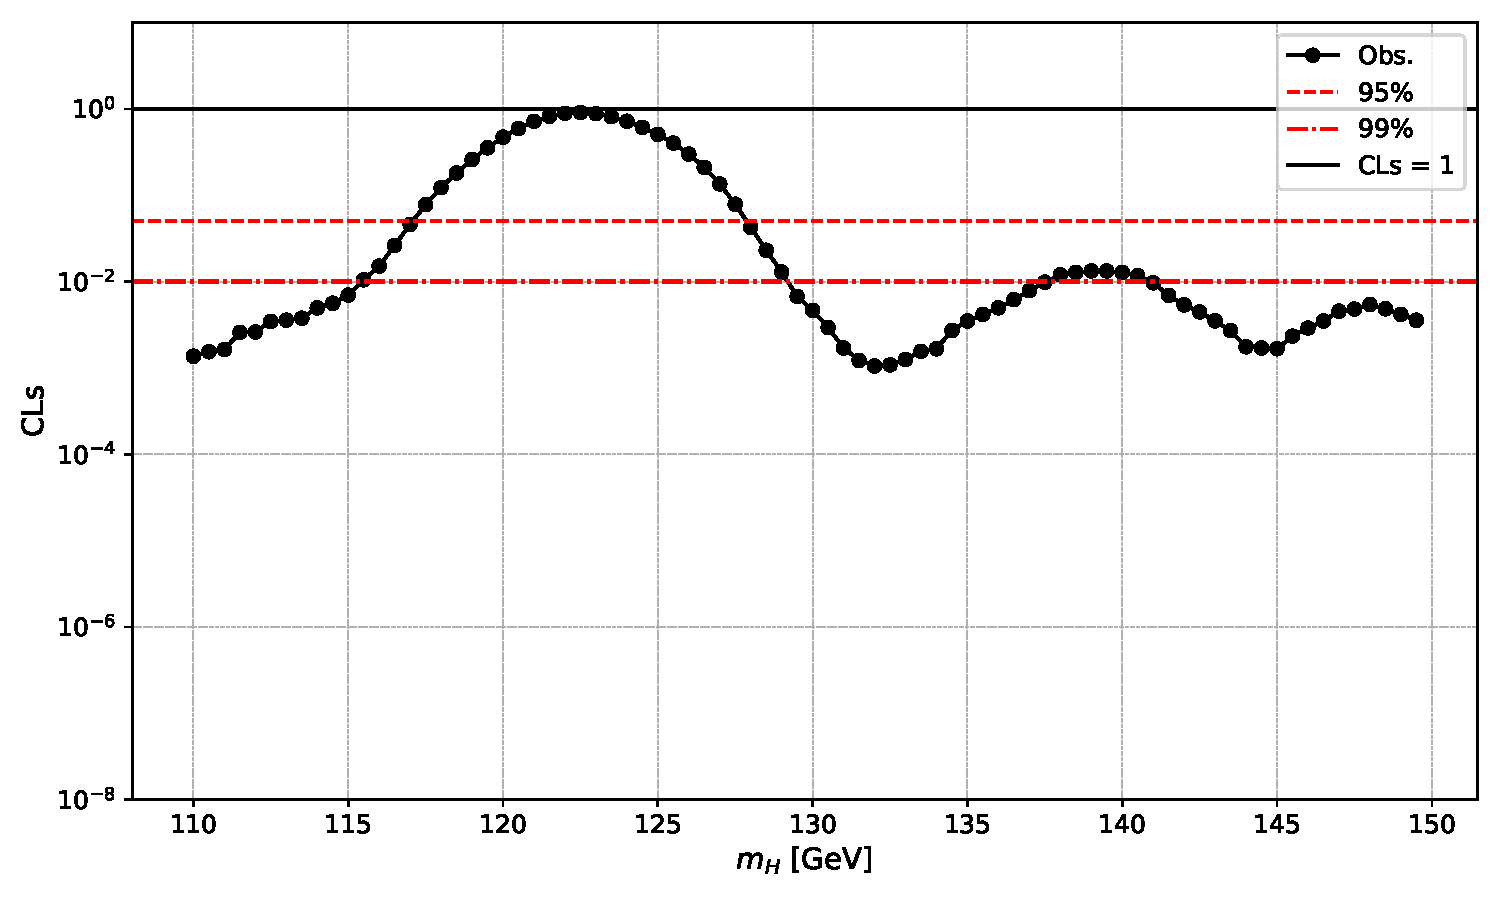
\includegraphics[scale=0.5]{images/clsEnhanced_small_nsig22/cls_plot.pdf}

Furthermore, it becomes much easier to do the larger peak dataset with $N_s = 45 \times \mu$, which gives us:

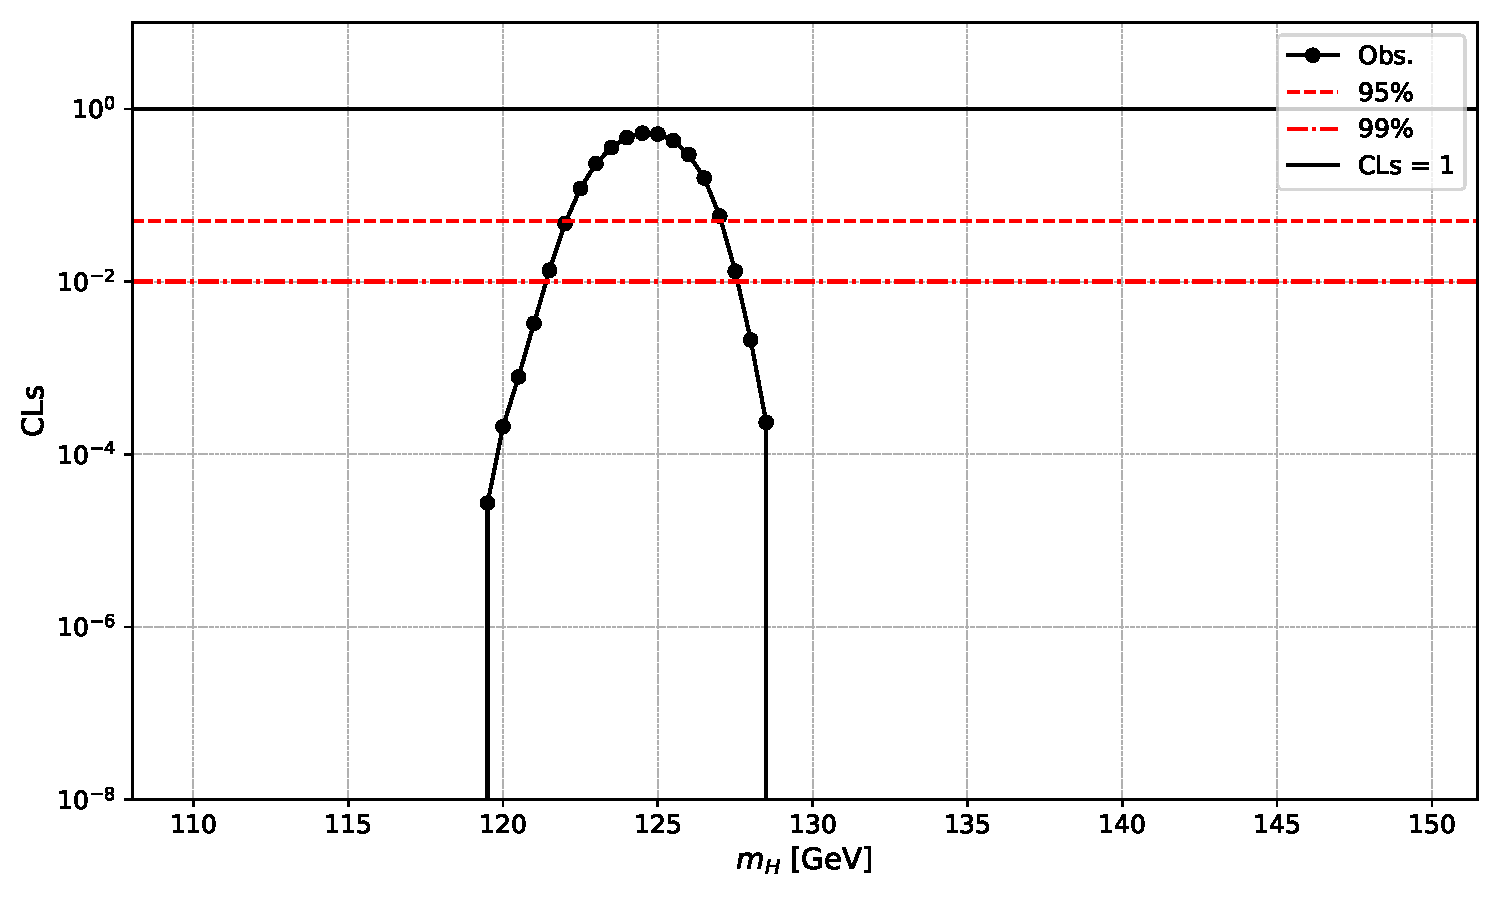
\includegraphics[scale=0.5]{images/clsEnhanced_large_nsig45/cls_plot.pdf}

\problempart{f}

The CLs method is a conservative limit on an exclusion confidence interval that modifies the confidence interval to not falsely exclude a region in the case where the experiement is simply just not sensitive to the signal. 

It is not a confidence interval because it is not purely frequentist, but instead weighted by the power of the test statistic. Instead, it is just an upper limit. 

\problempart{g}

When the number of observed signal events is large enough, the likelihood function will become a Gaussian and the CLs coverage will correctly cover a confidence interval. 






\end{document}